%----------------------------------------------------------------------------------------
%	PACKAGES AND DOCUMENT CONFIGURATIONS
%----------------------------------------------------------------------------------------

\documentclass{article}


\usepackage{graphicx} % Required for the inclusion of images
\graphicspath{{figures/}}
\usepackage{subfigure} % Required for the inclusion of images
\usepackage{natbib} % Required to change bibliography style to APA
\usepackage{amsmath} % Required for some math elements 
\usepackage{listings}
\usepackage{xcolor}
\usepackage{fontspec}
\usepackage{ctex}
\usepackage{geometry}
\geometry{a4paper,scale=0.8}
\renewcommand{\contentsname}{\centerline{目录}}
\setmonofont{Consolas}
\lstset{
basicstyle=\ttfamily\footnotesize,%
escapeinside=``,%
keywordstyle=\color{black},%\bfseries, \underbar,%
identifierstyle={},%
tabsize=4,
commentstyle=\color{blue},%
stringstyle=\ttfamily,%
%labelstyle=\tiny,%
extendedchars=false,%
linewidth=\textwidth,%
numbers=left,%
numberstyle=\tiny \color{blue},%
frame=trbl%
}
%点列
%\begin{itemize}
%\item[$\bullet$]Get familiar with Y86 assembly language.
%\end{itemize}

%小标题
%\begin{center}
%{\ttfamily rsum.ys}
%\end{center}
%代码
%\begin{lstlisting}[language={[ANSI]C}]
%\end{lstlisting}
%点列和浮动体图表和ref
%\begin{itemize}
%\item[$\bullet$]{\ttfamily sum.ys} (Figure \ref{Part A: sum.ys})\\
%\end{itemize}
%\begin{figure}[htbp]%figure浮动体环境 [htbp]指定位置
%		\centering%居中排版
%		\includegraphics{A_sum}
%		\caption{Part A  {\ttfamily sum.ys}} \label{Part A: sum.ys}%标题 自动编号 label标签
%\end{figure}


%\usepackage{times} % Uncomment to use the Times New Roman font

%----------------------------------------------------------------------------------------
%	DOCUMENT INFORMATION
%----------------------------------------------------------------------------------------

\title{\textbf{操作系统课程设计Project 5\\Designing a Thread Pool\\ \& Producer-Consumer Problem}} % Title

\author{姓名: 郭倩昀  
\\班级: F1903303  
\\学号: 519021910095  
\\Email: guoqianyun@sjtu.edu.cn} % Author name and email
\date{\today} % Date for the report
\begin{document}
\maketitle % Insert the title, author and date
\tableofcontents
\newpage
%%%%%%%%%%%%%%%%%%%%%%%%%%%%%%%%%%%%%
\section{Designing a Thread Pool}
\subsection{实验内容与目标}
本实验需要利用C语言创建并管理thread pool,根据提供的源文件Makefile以及client,threadpool文件,要求我们完善threadpool.c文件中的enqueue,dequeue,worker,pool\_submit,pool\_init,pool\_shutdown等函数。
\subsection{实验过程及步骤}
\begin{itemize}
\item[$\bullet$]将work queue设计为链接表\\
设计队列结点结构体并创建头结点和尾结点。
\item[$\bullet$]利用同步工具\\
创建mutex为访问work queue的时候避免竞争条件,创建信号量用于挂起等待线程。
\item[$\bullet$]完善enqueue与dequeue函数\\
enqueue根据传入的task创建queue node加入到任务列表,dequeue将头结点指向的任务删除并返回。
\item[$\bullet$]完善worker函数\\
work thread的工作函数,当有等待线程的时候将任务取出并执行,注意mutex和信号量的使用。结束后用pthread\_exit(0)返回。
\item[$\bullet$]完善pool\_submit函数\\
根据参数所给的函数信息和data信息创建task,加入到任务列表,注意mutex和信号量的使用。
\item[$\bullet$]完善pool\_init函数\\
线程池初始化时候,给任务列表头结点分配空间,初始化头结点和尾结点,初始化mutex和信号量,为每个线程调用pthread\_create创建线程并输出创建成功的信息。过程中用err记录关键步骤的执行情况,当出现错误时候及时报错并退出执行。
\item[$\bullet$]完善pool\_shutdown函数\\
将全局变量shutdown设为1,让线程不再继续接受新的任务。然后取消所有的信号量,等待线程执行完毕并输出执行完毕的信息,最后破坏mutex和信号量结束工作。
\item[$\bullet$]修改client.c文件便于测试\\
原来的client.c文件只有一个待完成的work,经修改后设定为随机生成10个work并递交给线程池工作。
\end{itemize}
\subsection{实验代码}
\begin{center}
{\ttfamily threadpool.c}
\end{center}
\begin{lstlisting}[language={[ANSI]C}]
/**
 * Implementation of thread pool.
 */

#include <pthread.h>
#include <stdlib.h>
#include <stdio.h>
#include <semaphore.h>
#include "threadpool.h"

#define QUEUE_SIZE 10
#define NUMBER_OF_THREADS 3

#define TRUE 1

// this represents work that has to be 
// completed by a thread in the pool
typedef struct 
{
    void (*function)(void *p);
    void *data;
}
task;

// the work queue
struct queue_node{	//linked list
	task worktodo;
	struct queue_node *next;
};
struct queue_node *head,*tail;


pthread_t bee[NUMBER_OF_THREADS];	// the worker bee
pthread_mutex_t queue_mutex;		//mutex
sem_t sem;				//semaphore
int shutdown;

// insert a task into the queue
// returns 0 if successful or 1 otherwise, 
int enqueue(task t) 
{
	tail->next=(struct queue_node *) malloc (sizeof(struct queue_node));
	if(tail->next==NULL) return 1;	//allocation error occurs
	tail=tail->next;				//add to the end
	tail->worktodo=t;
    return 0;
}

// remove a task from the queue
task dequeue() 
{
	if(head==tail)					//queue is empty
	{
		fprintf(stderr,"ERROR:no work to do\n");
		exit(1);
	}
	else
	{
		struct queue_node *tmp;		//remove from the head
		tmp=head;
		head=head->next;
		free(tmp);
	}
    return head->worktodo;
}

// the worker thread in the thread pool
void *worker(void *param)			//exe by each thread in the pool
{
	task tsk;
	while(TRUE)
	{
		sem_wait(&sem);				//notifying a waiting thread
		if(shutdown) break;
		pthread_mutex_lock(&queue_mutex);//avoid race conditions when accessing queue
		tsk=dequeue();
		pthread_mutex_unlock(&queue_mutex);
		execute(tsk.function, tsk.data);// execute the task
	}
    pthread_exit(0);
}

/**
 * Executes the task provided to the thread pool
 */
void execute(void (*somefunction)(void *p), void *p)
{
    (*somefunction)(p);
}

/**
 * Submits work to the pool.
 */
int pool_submit(void (*somefunction)(void *p), void *p)
{
	task tsk;		//place function and data
	tsk.function=somefunction;
	tsk.data=p;
	pthread_mutex_lock(&queue_mutex);//avoid race conditions when accessing queue
	int rst=enqueue(tsk);
	pthread_mutex_unlock(&queue_mutex);
	if(rst==0) sem_post(&sem);
    return rst;
}

// initialize the thread pool
void pool_init(void)
{
	int err;
	shutdown=0;
	head = (struct queue_node *) malloc (sizeof(struct queue_node));
	if(head==NULL)
	{
		fprintf(stderr,"ERROR:queue init error\n");
		exit(1);
	}
	head->next=NULL;
	tail=head;
	
	err=pthread_mutex_init(&queue_mutex,NULL);	//initialize mutex
	if(err)
	{
		fprintf(stderr,"ERROR:pthread mutex init error\n");
		exit(1);
	}
	err=sem_init(&sem,0,0);						//initialize semaphore
	if(err)
	{
		fprintf(stderr,"ERROR:semaphore init error\n");
		exit(1);
	}
	for(int i=0;i<NUMBER_OF_THREADS;i++)		//pthread create
	{
		err=pthread_create(&bee[i],NULL,worker,NULL);
		if(err)
		{
			fprintf(stderr,"ERROR:pthread create error\n");
			exit(1);
		}
	}
	fprintf(stdout,"Pthread create successfully\n");
}

// shutdown the thread pool
void pool_shutdown(void)
{
	int err;
	shutdown=1;
	for(int i=0;i<NUMBER_OF_THREADS;i++)		//cancel each worker thread
	{
		sem_post(&sem);
	}
	for(int i=0;i<NUMBER_OF_THREADS;i++)		//wait for each thread to terminate
	{
		err=pthread_join(bee[i],NULL);
		if(err)
		{
			fprintf(stderr,"ERROR:pthread join error\n");
			exit(1);
		}
	}
	fprintf(stdout,"Pthread join successfully\n");
	err=pthread_mutex_destroy(&queue_mutex);	//destroy mutex
    if(err)
	{
		fprintf(stderr,"ERROR:pthread mutex destroy error\n");
		exit(1);
	}
	err=sem_destroy(&sem);						//destroy semaphore
	if(err)
	{
		fprintf(stderr,"ERROR:semaphore destroy error\n");
		exit(1);
	}
}
\end{lstlisting}
\begin{center}
{\ttfamily client.c}
\end{center}
\begin{lstlisting}[language={[ANSI]C}]
/**
 * Example client program that uses thread pool.
 */

#include <stdlib.h>
#include <stdio.h>
#include <unistd.h>
#include <time.h>
#include "threadpool.h"

struct data
{
    int a;
    int b;
};

void add(void *param)
{
    struct data *temp;
    temp = (struct data*)param;

    printf("I add two values %d and %d result = %d\n",temp->a, temp->b, temp->a + temp->b);
}

int main(void)
{
	
    // create some work to do
    srand((unsigned)time(NULL));
	struct data work[10];
	for (int i = 0; i < 10; ++ i) {
		work[i].a = rand() % 100;
		work[i].b = rand() % 100;
	}


    // initialize the thread pool
    pool_init();

    // submit the work to the queue
	for (int i = 0; i < 10; ++ i) {
		static int err;
		err = pool_submit(&add, &work[i]);
		if (err) 
		fprintf(stderr, "Submit work %d error because the task queue is full.\n", i);
	}

    sleep(3);

    pool_shutdown();

    return 0;
}
\end{lstlisting}
\subsection{实验测试}
\begin{itemize}
\item[$\bullet$]thread pool测试 (图 \ref{thread pool测试})
\begin{figure}[htbp]
		\centering
		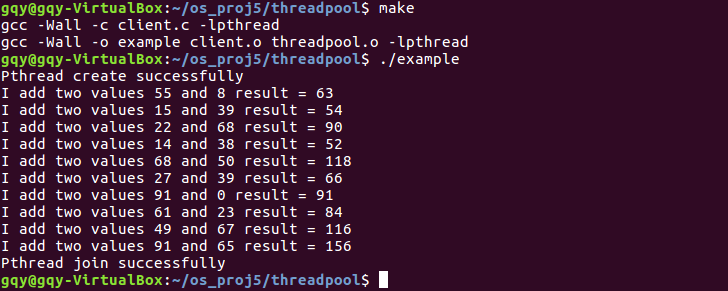
\includegraphics{tp}
		\caption{thread pool测试} \label{thread pool测试}
\end{figure}

测试指令如下
\begin{lstlisting}[language={[ANSI]C}]
make
./example
\end{lstlisting}
首先用Makefile文件编译,生成example可执行文件,输入./example并执行,测试生成的10个work递交给线程池工作,测试结果如图 \ref{thread pool测试}。
\end{itemize}
%%%%%%%%%%%%%%%%%%%%%%%%%%%%%%%%%%%%%%%%%
\section{Producer-Consumer Problem}
\subsection{实验内容与目标}
本实验需要利用C语言结合mutex,信号量和线程使用应对生产者-消费者问题。需要设计buffer以及producer\_consumer.c文件实现,参考书本7.1.1的方式利用同步工具,针对每一个生产者和消费者创建相应的线程工作。
\subsection{实验过程及步骤}
\begin{itemize}
\item[$\bullet$]buffer设计\\
根据书本指导,设计的buffer包含函数insert\_item(),remove\_item(),另外添加了一个初始化函数buffer\_init()。buffer的数组大小设为比规定大小多一位,头指针和尾指针分别指向buffer中第一个元素的前一位以及最后一个元素。初始化函数将头指针和尾指针设为0。insert\_item将元素插入到尾指针后并更新尾指针,remove\_item将头指针的元素传出,如果遇到buffer满或空导致不能进行加减元素则返回$-1$表示异常。
\item[$\bullet$]同步工具的使用\\
producer\_consumer.c中创建mutex和信号量empty和full。mutex用于在访问buffer的时候避免竞争条件。empty和full用于挂起等待的消费者或者生产者线程。empty初始化为BUFFER\_SIZE,full初始化为0。
\item[$\bullet$]为生产者和消费者设计线程工作函数\\
每个生产者每次间隔随机时间,然后生成随机item并通过insert\_item加入到buffer中;每个消费者每次间隔随机时间,然后通过remove\_item从buffer中消费item。注意中间的mutex和信号量的使用,工作时如果终止信号terminate为1则停止工作退出,如果出现错误情况及时报错。结束工作后调用pthread\_exit(0)退出。
\item[$\bullet$]main()函数设计\\
首先通过命令行读入三个参数,分别为终止前运行时间,生产者个数和消费者个数。然后分别初始化buffer,mutex,full,empty(注意初始值设置),为每一个生产者和消费者线程分配空间并调用pthread\_create创建并输出创建成功的信息,传入工作函数。运行时间结束后将终止信号terminate设为1,让所有线程停止工作并退出,调用pthread\_join等待线程结束工作并输出结束信息,最后破坏mutex和信号量结束工作。
\end{itemize}
\subsection{实验代码}
\begin{center}
{\ttfamily buffer.h}
\end{center}
\begin{lstlisting}[language={[ANSI]C}]
/* buffer.h */
typedef int buffer_item;
#define BUFFER_SIZE 5
int insert_item(buffer_item item);
int remove_item(buffer_item *item);
void buffer_init();
\end{lstlisting}
\begin{center}
{\ttfamily buffer.c}
\end{center}
\begin{lstlisting}[language={[ANSI]C}]
# include "buffer.h"

buffer_item buffer[BUFFER_SIZE+1];
int head;//before the first one in the buffer
int tail;//last one in the buffer

void buffer_init()				//buffer initialize
{
	head=0;
	tail=0;
}

int insert_item(buffer_item item)
{
	if((tail+1)%(BUFFER_SIZE+1)==head)	//full
		return -1;
	tail = (tail+1)%(BUFFER_SIZE+1);
	buffer[tail]=item;
	return 0;
}

int remove_item(buffer_item *item)
{
	if(head==tail)				//empty
		return -1;
	head=(head+1)%(BUFFER_SIZE+1);
	*item=buffer[head];
	return 0;
}
\end{lstlisting}

\begin{center}
{\ttfamily producer\_consumer.c}
\end{center}
\begin{lstlisting}[language={[ANSI]C}]
#include <stdio.h>
#include <unistd.h>
#include <stdlib.h>
#include <time.h>
#include <pthread.h>
#include <semaphore.h>
#include "buffer.h"

#define TRUE 1
#define RANDOM_TIME_BASE 5
int terminate;
pthread_mutex_t mutex;//for accessing buffer
sem_t empty, full;

void *producer(void *param);

void *consumer(void *param);

int main(int argc, char *argv[]){
	srand((unsigned)time(NULL));
	
	terminate=0;
	pthread_t *producer_t, *consumer_t;
	int time, producer_number, consumer_number;
	static int err;
	
//get command line
	if(argc!=4)
	{
		fprintf(stderr,"ERROR:invalid arguments\n");
		exit(1);
	}
	time=atoi(argv[1]);
	producer_number=atoi(argv[2]);
	consumer_number=atoi(argv[3]);
	
//initialize the buffer
	buffer_init();
	
	//initialize the mutex lock
	err=pthread_mutex_init(&mutex, NULL);
	if(err)
	{
		fprintf(stderr,"ERROR:pthread mutex init create error\n");
		exit(1);
	}
	
	//initialize the semaphore
	err=sem_init(&empty, 0, BUFFER_SIZE);//empty initialize to n
	if(err)
	{
		fprintf(stderr,"ERROR:semaphore init create error\n");
		exit(1);
	}
	err=sem_init(&full, 0, 0);//full initialize to 0
	if(err)
	{
		fprintf(stderr,"ERROR:semaphore init create error\n");
		exit(1);
	}
	
//create producer threads
	producer_t = (pthread_t*)malloc(sizeof(pthread_t)*producer_number);
	for(int i=0;i<producer_number;i++)
	{
		pthread_create(&producer_t[i],NULL,&producer,NULL);
	}
	
//create consumer threads
	consumer_t = (pthread_t*)malloc(sizeof(pthread_t)*consumer_number);
	for(int i=0;i<consumer_number;i++)
	{
		pthread_create(&consumer_t[i],NULL,&consumer,NULL);
	}
	fprintf(stdout,"Pthread create successfully\n");
//sleep
	sleep(time);
	
//terminate
	terminate=1;
	//cancel each thread
	for(int i=0;i<producer_number;i++)
	{
		sem_post(&empty);
	}
	for(int i=0;i<consumer_number;i++)
	{
		sem_post(&full);
	}
	//pthread join
	for(int i=0;i<producer_number;i++)
	{
		err=pthread_join(producer_t[i],NULL);
		if(err)
		{
			fprintf(stderr,"ERROR:pthread join error\n");
			exit(1);
		}
	}
	for(int i=0;i<consumer_number;i++)
	{
		err=pthread_join(consumer_t[i],NULL);
		if(err)
		{
			fprintf(stderr,"ERROR:pthread join error\n");
			exit(1);
		}
	}
	fprintf(stdout,"Pthread join successfully\n");
	
	//destroy mutex
	err=pthread_mutex_destroy(&mutex);	
    if(err)
	{
		fprintf(stderr,"ERROR:pthread mutex destroy error\n");
		exit(1);
	}
	
	//destroy semaphore
	err=sem_destroy(&empty);						
	if(err)
	{
		fprintf(stderr,"ERROR:semaphore destroy error\n");
		exit(1);
	}
	err=sem_destroy(&full);						
	if(err)
	{
		fprintf(stderr,"ERROR:semaphore destroy error\n");
		exit(1);
	}
	free(producer_t);
	free(consumer_t);
	
	return 0;
}

void *producer(void *param)
{
	buffer_item item;
	while(TRUE)
	{
		//sleep for a random period of time
		int random_time;
		random_time=rand()%RANDOM_TIME_BASE;
		sleep(random_time);
		
		//generate a random number
		item=rand();
		
		sem_wait(&empty);
		pthread_mutex_lock(&mutex);
		if(terminate) break;
		if(insert_item(item))
			fprintf(stderr,"ERROR: cannot insert item %d\n", item);
		else
			fprintf(stdout,"Producer produced item %d\n", item);
		pthread_mutex_unlock(&mutex);
		sem_post(&full);
	}
	pthread_mutex_unlock(&mutex);
	pthread_exit(0);
}

void *consumer(void *param)
{
	buffer_item item;
	while(TRUE)
	{
		//sleep for a random period of time
		int random_time;
		random_time=rand()%RANDOM_TIME_BASE;
		sleep(random_time);
		
		sem_wait(&full);
		pthread_mutex_lock(&mutex);
		if(terminate) break;
		if(remove_item(&item))
			fprintf(stderr,"ERROR: cannot remove item %d\n", item);
		else
			fprintf(stdout,"Consumer consumed item %d\n", item);
		pthread_mutex_unlock(&mutex);
		sem_post(&empty);
	}
	pthread_mutex_unlock(&mutex);
	pthread_exit(0);
}
\end{lstlisting}
\begin{figure}[htbp]
		\centering
		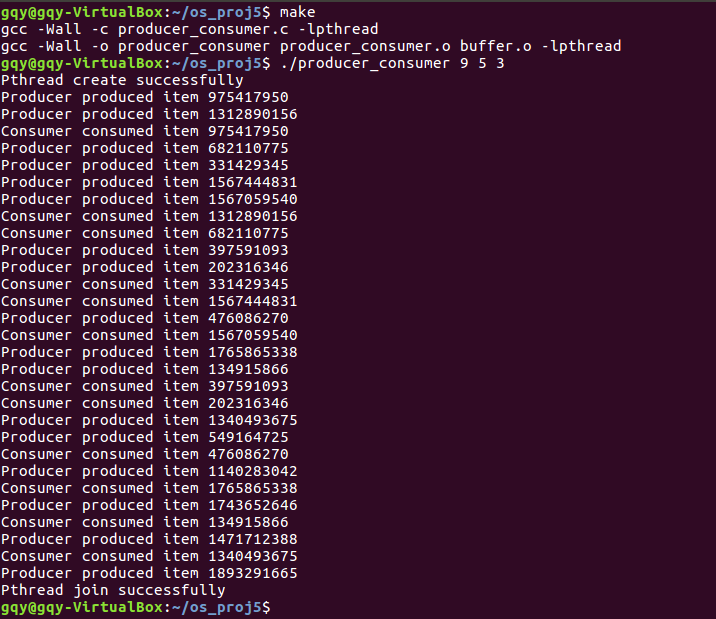
\includegraphics{pc}
		\caption{producer consumer测试} \label{producer consumer测试}
\end{figure}
\subsection{实验测试}
\begin{itemize}
\item[$\bullet$]producer consumer测试 (图 \ref{producer consumer测试})
测试指令如下
\begin{lstlisting}[language={[ANSI]C}]
make
./producer_consumer 9 5 3
\end{lstlisting}
首先用Makefile文件编译,生成可执行文件producer\_consumer,输入运行时间9s,生产者5个,消费者3个并执行,测试结果如图 \ref{producer consumer测试}。
\end{itemize}
%%%%%%%%%%%%%%%%%%%%%%%%%%%%%%%%%%%%%%%%%%%
\section{Conclusion}

\subsection{问题与解决方案}
由于经过project4后对线程应用比较熟悉,本次project对线程的应用难度不大,主要困难点就在于同步工具的使用,包括mutex和信号量的使用,需要对同步工具有透彻的理解并清楚了解程序中每一个创建的同步工具的具体用处,并正确运用。原本理论学习的时候对这些同步工具的理解并没有那么深入,在本次project设计中重新仔细阅读书上的示例并经过多次尝试后成功正确应用了同步工具完成了实验内容。

\subsection{实验心得}
本次project5让我进一步熟悉了线程的运用,与此同时增加了同步工具的使用,让我对mutex,信号量等工具有了更清晰的认识。虽然由于运用不熟练过程中出现了一些错误,但是最终多次尝试后调试成功,可以见得除了理论学习外,最终还是要多动手亲自来实现才可以真正掌握新的知识和工具。总的来说本次project很好地锻炼了代码能力并加深了对进程同步工具的理解,让我受益匪浅。




%----------------------------------------------------------------------------------------


\end{document}